\documentclass{article}
\usepackage[utf8]{inputenc}
\usepackage{listings}
\usepackage{multimedia} % to embed movies in the PDF file
\usepackage{graphicx}
\usepackage{comment}
\usepackage[english]{babel}
\usepackage{amsmath}
\usepackage{amsfonts}
\usepackage{subfigure}
\usepackage{wrapfig}
\usepackage{multirow}
\usepackage{tikz}
\usepackage{verbatim}

\newtheorem{theorem}{Theorem}[section]
\newtheorem{lemma}[theorem]{Lemma}
\newtheorem{corollary}[theorem]{Corollary}
%\newtheorem{algorithm}[theorem]{Algorithm}
\newtheorem{remark}[theorem]{Remark}
\newenvironment{proof}{\noindent {\bf Proof:} }{\hfill $\Box$ \\[2ex] }
\newenvironment{keywords}{\begin{quote} {\bf Key words} }
                         {\end{quote} }
\newenvironment{AMS}{\begin{quote} {\bf AMS subject classifications} }
                         {\end{quote} }


\newcommand{\eref}[1]{\mbox{\rm(\ref{#1})}}
\newcommand{\tref}[1]{\mbox{\rm\ref{#1}}}
\newcommand{\set}[2]{\left\{ #1 \; : \; #2 \right\} }
\newcommand{\deq}{\raisebox{0pt}[1ex][0pt]{$\stackrel{\scriptscriptstyle{\rm def}}{{}={}}$}}

\newcommand {\DS} {\displaystyle}

\newcommand{\real}{\mathbb{R}}
\newcommand{\compl}{\mathbb{C}}



\newcommand {\half} {\mbox{$\frac{1}{2}$}}
\newcommand{\force}{{\mathbf{f}}}
\newcommand{\strain}{{\boldsymbol{\varepsilon}}}
\newcommand{\stress}{{\boldsymbol{\sigma}}}
\renewcommand{\div}{{\boldsymbol{\nabla}}}

\newcommand {\cA} {{\cal A}}
\newcommand {\cB} {{\cal B}}
\newcommand {\cC} {{\cal C}}
\newcommand {\cD} {{\cal D}}
\newcommand {\cE} {{\cal E}}
\newcommand {\cL} {{\cal L}}
\newcommand {\cP} {{\cal P}}
\newcommand {\cQ} {{\cal Q}}
\newcommand {\cR} {{\cal R}}
\newcommand {\cV} {{\cal V}}
\newcommand {\cW} {{\cal W}}
\newcommand {\CH} {{\cal H}}
\newcommand {\CS} {{\cal S}}


\newcommand{\bzero}{\mathbf{0}}
\newcommand{\ba}{\mathbf{a}}
\newcommand{\bb}{\mathbf{b}}
\newcommand{\bc}{\mathbf{c}}
\newcommand{\bd}{\mathbf{d}}
\newcommand{\be}{\mathbf{e}}
\newcommand{\bff}{\mathbf{f}}
\newcommand{\bg}{\mathbf{g}}
\newcommand{\bh}{\mathbf{h}}
\newcommand{\bn}{\mathbf{n}}
\newcommand{\bp}{\mathbf{p}}
\newcommand{\bq}{\mathbf{q}}
\newcommand{\br}{\mathbf{r}}
\newcommand{\bs}{\mathbf{s}}
\newcommand{\bt}{\mathbf{t}}
\newcommand{\bu}{\mathbf{u}}
\newcommand{\bv}{\mathbf{v}}
\newcommand{\bw}{\mathbf{w}}
\newcommand{\bx}{\mathbf{x}}
\newcommand{\by}{\mathbf{y}}
\newcommand{\bz}{\mathbf{z}}
\newcommand{\bA}{\mathbf{A}}
\newcommand{\bB}{\mathbf{B}}
\newcommand{\bC}{\mathbf{C}}
\newcommand{\bD}{\mathbf{D}}
\newcommand{\bE}{\mathbf{E}}
\newcommand{\bF}{\mathbf{F}}
\newcommand{\bG}{\mathbf{G}}
\newcommand{\bH}{\mathbf{H}}
\newcommand{\bI}{\mathbf{I}}
\newcommand{\bJ}{\mathbf{J}}
\newcommand{\bK}{\mathbf{K}}
\newcommand{\bL}{\mathbf{L}}
\newcommand{\bM}{\mathbf{M}}
\newcommand{\bN}{\mathbf{N}}
\newcommand{\bO}{\mathbf{O}}
\newcommand{\bP}{\mathbf{P}}
\newcommand{\bQ}{\mathbf{Q}}
\newcommand{\bR}{\mathbf{R}}
\newcommand{\bS}{\mathbf{S}}
\newcommand{\bU}{\mathbf{U}}
\newcommand{\bV}{\mathbf{V}}
\newcommand{\bW}{\mathbf{W}}
\newcommand{\bX}{\mathbf{X}}
\newcommand{\bY}{\mathbf{Y}}
\newcommand{\bZ}{\mathbf{Z}}

\newcommand{\cO}{ {\cal O} }
\newcommand{\CT}{ {\cal T} }
\newcommand{\IL}{{\mathbb L}}
\newcommand{\sIL}{{{{\mathbb L}_s}}}
\newcommand{\bOmega}{{\boldsymbol{\Omega}}}
\newcommand{\bPsi}{{\boldsymbol{\Psi}}}

\newcommand{\bgamma}{{\boldsymbol{\gamma}}}
\newcommand{\bmu}{{\boldsymbol{\mu}}}
\newcommand{\blambda}{{\boldsymbol{\lambda}}}
\newcommand{\bLambda}{{\boldsymbol{\Lambda}}}
\newcommand{\bpi}{{\boldsymbol{\pi}}}
\newcommand{\bPi}{{\boldsymbol{\Pi}}}
\newcommand{\bphi}{{\boldsymbol{\phi}}}
\newcommand{\bPhi}{{\boldsymbol{\Phi}}}
\newcommand{\bpsi}{{\boldsymbol{\psi}}}
\newcommand{\btheta}{{\boldsymbol{\theta}}}
\newcommand{\bTheta}{{\boldsymbol{\Theta}}}
\newcommand{\bSigma}{{\boldsymbol{\Sigma}}}
\newcommand{\sump}{\sideset{}{^{'}}\sum} 
\DeclareMathOperator*{\Res}{Res}
\DeclareMathOperator{\OO}{O}
\DeclareMathOperator{\oo}{o}
\DeclareMathOperator{\erfc}{erfc}
\def\Xint#1{\mathchoice
   {\XXint\displaystyle\textstyle{#1}}%
   {\XXint\textstyle\scriptstyle{#1}}%
   {\XXint\scriptstyle\scriptscriptstyle{#1}}%
   {\XXint\scriptscriptstyle\scriptscriptstyle{#1}}%
   \!\int}
\def\XXint#1#2#3{{\setbox0=\hbox{$#1{#2#3}{\int}$}
     \vcenter{\hbox{$#2#3$}}\kern-.5\wd0}}
\def\ddashint{\Xint=}
\def\pvint{\Xint-}





\title{AMATH 570 Homework 3}
\author{Cade Ballew}
\date{November 1, 2021}

\begin{document}

\maketitle

\section{Problem 1}
\subsection{Exercise 5.1}
\subsubsection{Part a}
Given interpolation points $x_0=-1$, $x_1=0$, $x_2=1/2$, and $x_3=1$, we find the barycentric interpolation coefficients.
\begin{align*}
\lambda_0=\frac{1}{(-1)(-1-1/2)(-1-1)}&=\frac{-1}{3}\\
\lambda_1=\frac{1}{(1)(-1/2)(-1)}&=2\\
\lambda_2=\frac{1}{(1/2+1)(1/2)(1/2-1)}&=\frac{-8}{3}\\
\lambda_3=\frac{1}{(1+1)(1)(1-1/2)}&=1
\end{align*}
\subsubsection{Part b}
Now, we verify that (5.9) in ATAP gives the same result as standard polynomial interpolation via (5.3) at $x=-1/2$. First, compute
\[
\ell(-1/2)=(-1/2+1)(-1/2)(-1/2-1/2)(-1/2-1)=\frac{-3}{8}.
\]
Also,
\begin{align*}
\frac{\lambda_0}{-1/2-x_0}=\frac{-1/3}{1/2}&=\frac{-2}{3}\\
\frac{\lambda_1}{-1/2-x_1}=\frac{2}{-1/2}&=-4\\
\frac{\lambda_2}{-1/2-x_2}=\frac{-8/3}{-1}&=\frac{8}{3}\\
\frac{\lambda_3}{-1/2-x_3}=\frac{1}{-3/2}&=\frac{-2}{3}
\end{align*}
Finally, we get that 
\begin{align*}
\ell_0(-1/2)=\frac{-3}{8}\frac{-2}{3}&=\frac{1}{4}\\
\ell_1(-1/2)=\frac{-3}{8}(-4)&=\frac{3}{2}\\
\ell_2(-1/2)=\frac{-3}{8}\frac{8}{3}&=-1\\
\ell_3(-1/2)=\frac{-3}{8}\frac{-2}{3}&=\frac{1}{4}.
\end{align*}
Now, we compute these same values in the normal manner
\begin{align*}
\ell_0(-1/2)=\frac{(-1/2)(-1/2-1/2)(-1/2-1)}{(-1)(-1-1/2)(-1-1)}=\frac{-3/4}{-3}&=\frac{1}{4}\\
\ell_1(-1/2)=\frac{(-1/2+1)(-1/2-1/2)(-1/2-1)}{(1)(-1/2)(-1)}=\frac{3/4}{1/2}&=\frac{3}{2}\\
\ell_2(-1/2)=\frac{(-1/2+1)(-1/2)(-1/2-1)}{(1/2+1)(1/2)(1/2-1)}=\frac{3/8}{-3/8}&=-1\\
\ell_3(-1/2)=\frac{(-1/2+1)(-1/2)(-1/2-1/2)}{(1+1)(1)(1-1/2)}=\frac{1/4}{1}&=\frac{1}{4}.
\end{align*}
Clearly, these values are identical.
\subsection{Exercise 5.2}
For the function $f(x)=\cos{kx}$, we use MATLAB to compute the value of various interpolants (chebfun, polyfit, and polyfitA) as well as the condition number of Vandermonde matrix used by polyfit for various values of k and obtain the results
\begin{verbatim}
            Chebfun           polyfit         polyfitA     condition number
k=10:                1     1.000000e+00     1.000000e+00     8.506226e+12
k=20:     1.000000e+00     1.000000e+00     1.000000e+00     6.676559e+16
k=30:     1.000000e+00     9.999932e-01                1     2.615273e+17
k=40:     1.000000e+00     9.919971e-01     1.000000e+00     6.059928e+18
k=50:     1.000000e+00     5.934477e-01     1.000000e+00     6.469850e+18
k=60:     1.000000e+00    -2.137573e-01     1.000000e+00     7.351968e+18
k=70:     1.000000e+00    -1.448931e-02     1.000000e+00     8.177436e+18
k=80:     1.000000e+00     3.892366e-02     1.000000e+00     1.005588e+19
k=90:     1.000000e+00     4.893440e-02     1.000000e+00     2.872486e+19
k=100:     1.000000e+00     2.043693e-02     1.000000e+00     7.184542e+18
\end{verbatim}
See problem5\_2.m for the code that produces this table.
\subsection{Exercise 5.7}
Using a greedy algorithm to determine the interpolation points for the function $f(x)=|x|$, we obtain the following error plots\\
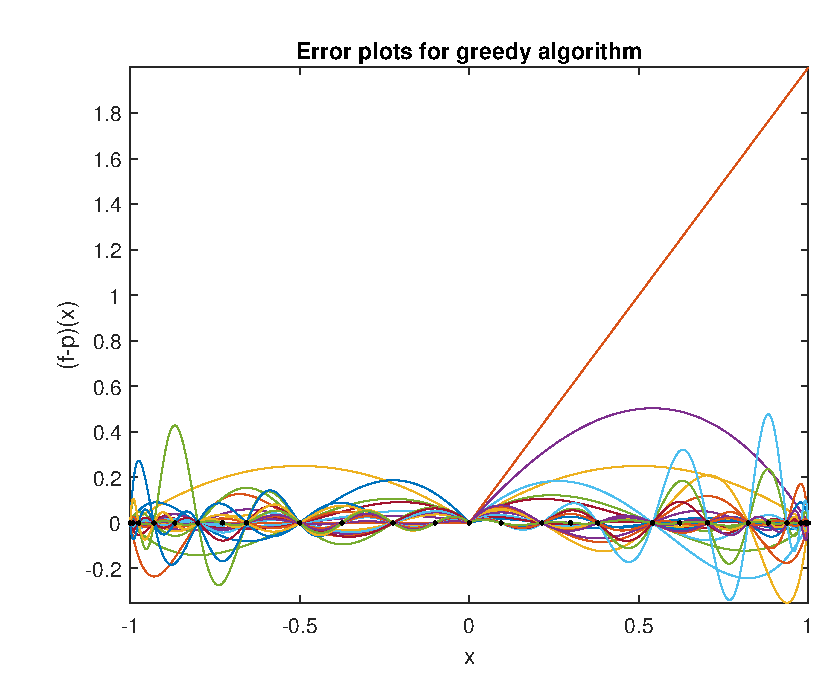
\includegraphics[scale=0.7]{prob5-7a.eps}\\
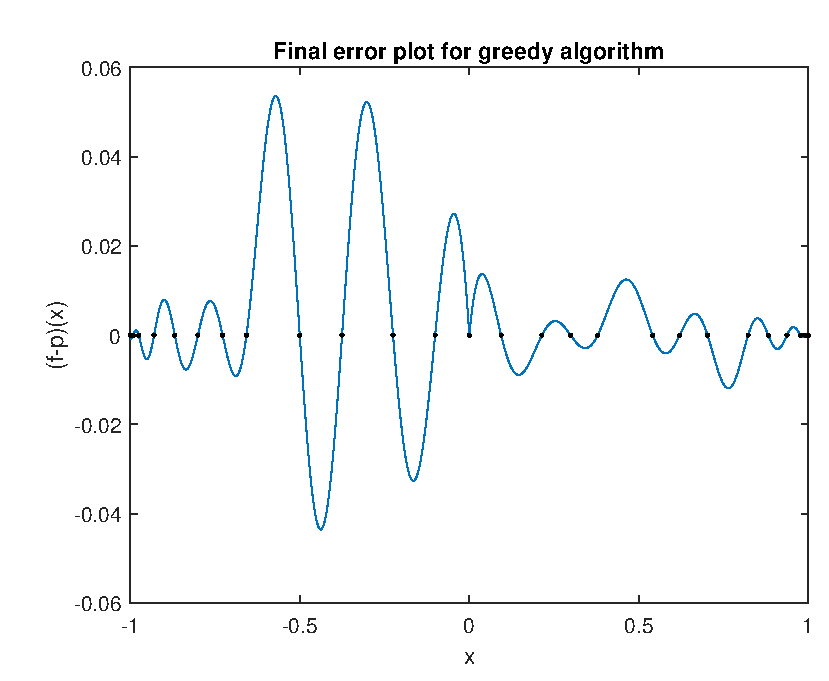
\includegraphics[scale=0.7]{prob5-7b.eps}\\
where the first includes the error plots for all interpolants used throughout the algorithm, and the second is just the final error plot for $n=25$. Looking at the spacing of the grid, the chosen points look quite similar to the Chebyshev points, but as one can check using chebfun, are not the Chebyshev points exactly. \\
See problem5\_7.m for the code that does this.

\section{Problem 2 (Exercise 6.3)} 
We compute the Chebyshev interpolant of $f(x) = \sin(1/x) \sin(1/ \sin(1/x))$ on the interval $[0.07,0.4]$ for various values of n and plot the errors. \\
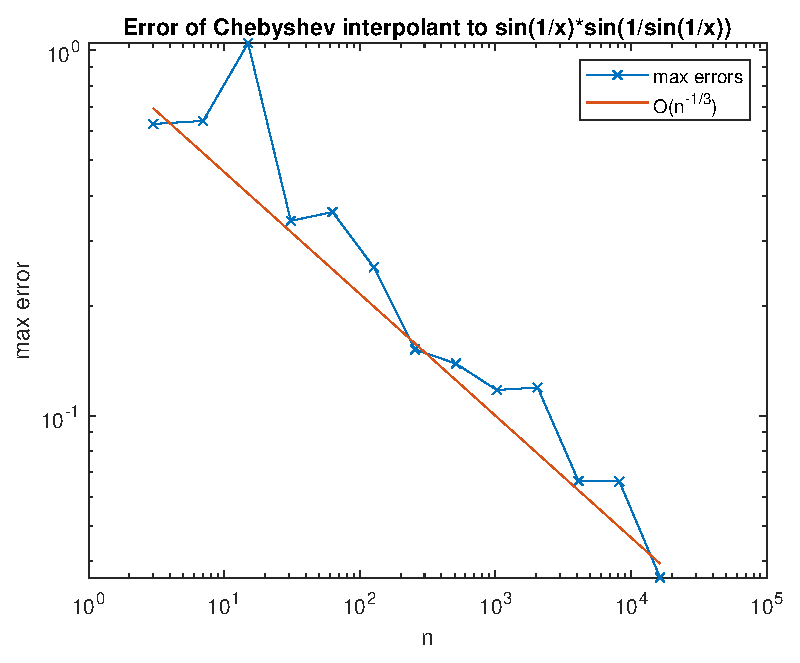
\includegraphics[]{prob6-3.eps}\\
We can see that the convergence appears to be roughly $O(n^{-1/3})$ which implies that in order to get accuracy around $10^{-16}$, we need $n$ to roughly be $10^{48}$.\\
See problem6\_3.m for the code that does this.

\section{Problem 3 (Exercise 7.1)}
\subsection{Part a}
Using chebfun to compute the total variation of $f(x) =\sin(100x)/(1 + x^2)$ on $[-1,1]$, we get that it is roughly 99.836. See problem7\_1.m for the code that does this.
\subsection{Part b}
To see that the total variation of $f(x) =\sin(Mx)/(1 + x^2)$ on $[-1,1]$ is asymptotic to $M$ as $M\to\infty$, first write out the definition of total variation
\[
\int_{-1}^1\left|\left(\frac{\sin(Mx)}{1 + x^2}\right)'\right|dx=\int_{-1}^1\left|\frac{(1+x^2)M\cos(Mx)-2x\sin(Mx)}{(1 + x^2)^2}\right|dx
\].
Now, consider that
\[\int_{-1}^1\left|\frac{2x\sin(Mx)}{1+x^2}\right|dx\leq\int_{-1}^1\left|\frac{2x}{1+x^2}\right|dx=1
\]
because $|\sin(Mx)|\leq1$. Thus, this term becomes negligible as $M\to\infty$, so we can consider only
\[
M\int_{-1}^1\left|\frac{\cos(Mx)}{1 + x^2}\right|dx
\]
The key observation here is that $|\cos(Mx)|$ rapidly oscillates as $M\to\infty$, so its average over any region will tend to its average over a period. Over a given period, it will have average \[
\frac{1}{\pi/M}\int_{-\pi/2M}^{\pi/2M}|\cos(Mx)|dx=\frac{M}{\pi}\left[\frac{\sin(Mx)}{M}\right]_{-\pi/2M}^{\pi/2M}=\frac{2}{\pi}.
\]
From this, we can infer that the total variation as $M\to\infty$ looks like 
\[
M\int_{-1}^1\frac{2/\pi}{1 + x^2}dx=\frac{2M}{\pi}\int_{-1}^1\frac{dx}{1+x^2}=\frac{2M}{\pi}\frac{\pi}{2}=M.
\]

\section{Problem 4}
\subsection{Exercise 8.1}
Consider a Bernstein ellipse $E_\rho$ where $\rho>1$. We know that $E_\rho$ is the circle $z=\rho e^{i\theta}$ under the Joukowsky map, so to find the rightmost endpoint of the ellipse, we need to find the $\theta$ that maximizes the real part of $\frac{1}{2}(\rho e^{i\theta}+\frac{1}{\rho e^{i\theta}})$. This is precisely $\theta=0$, because that is the value of $\theta$ (ignoring periodicity) that maximizes the real part of $\rho e^{i\theta}$. Thus, the rightmost endpoint is given by $\frac{1}{2}(\rho+\frac{1}{\rho})$. Similarly, the uppermost endpoint of the ellipse is given by the point that maximizes the imaginary part which is $\theta=\pi/2$, so the uppermost endpoint is given by $\frac{i}{2}(\rho-\frac{1}{\rho})$. Of course, the ellipse is centered at the origin, so clearly the length of the semimajor axis is $\frac{1}{2}(\rho+\frac{1}{\rho})$ and the length of the semiminor axis is $\frac{1}{2}(\rho-\frac{1}{\rho})$, so their sum is $\rho$.

\subsection{Exercise 8.3}
Consider $f(x)=\exp(-x^2)$. Because it is entire, we can apply Theorem 8.2 for any positive $\rho$, but must choose $M$ to be the maximum value that $f$ takes on $E_\rho$. For this choice of $f$, this occurs on the top (or bottom) of the ellipse, so we take 
\[
M=e^{-(i\frac{\rho-\rho^{-1}}{2})^2}=e^{(\frac{\rho-\rho^{-1}}{2})^2}.
\]
Plotting error against the bound given in the theorem for various values of $\rho$, we get\\
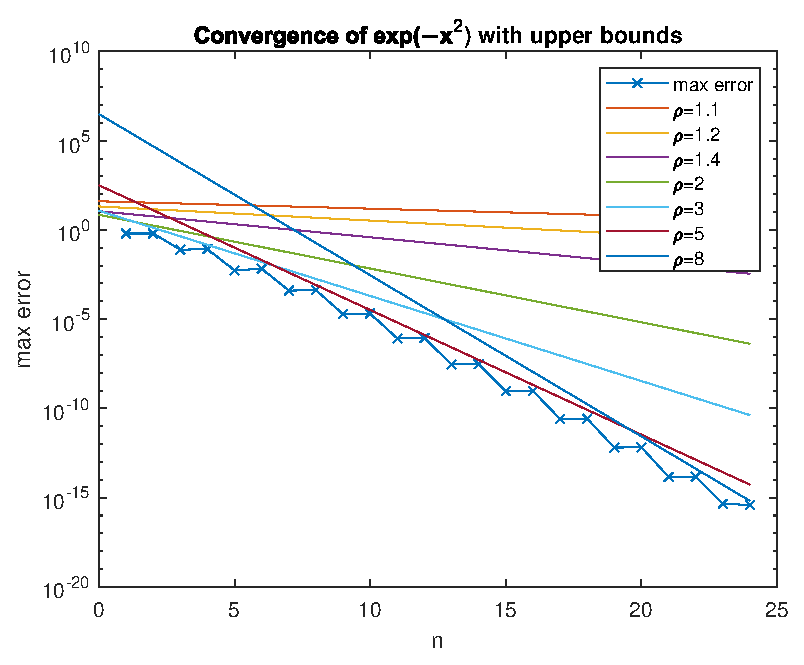
\includegraphics[]{prob8-3.eps}\\
For high values of $\rho$, this bound is pretty tight, but the bound does not fit the data very well for low values of $\rho$.

\section{Problem 5}
Assume $0 < m < M$ and let $\kappa = M/m$.  Consider the $k$th scaled and shifted
Chebyshev polynomial:
\begin{equation*}
T_k \left( \frac{2x - M - m}{M - m} \right) / T_k \left( \frac{-M-m}{M-m} \right) .
\end{equation*}
The numerator is shifted so that the interval $[m,M]$ maps linearly to $[-1,1]$. We know that a Chebyshev polynomial $T_k$ satisfies $-1\leq T_k(x)\leq1$ for $x\in[-1,1]$, so we can bound $\left|T_k \left( \frac{2x - M - m}{M - m} \right)\right|\leq1$ for $x\in[m,M]$. Looking at the denominator,
\[
T_k \left( \frac{-M-m}{M-m} \right)=T_k \left( -\frac{\frac{M}{m}+1}{\frac{M}{m}-1} \right)=T_k \left(- \frac{\kappa+1}{\kappa-1} \right).
\]
Per the hint, we now look to find a $z$ such that $\frac{1}{2}(z+z^{-1}=- \frac{\kappa+1}{\kappa-1})$. This yields a quadratic equation $z^2+2\frac{\kappa+1}{\kappa-1}z+1=0$ which has solution
\[
z=-\frac{\kappa+1}{\kappa-1}\pm\sqrt{\left(\frac{\kappa+1}{\kappa-1}\right)^2-1}=-\frac{\kappa+1}{\kappa-1}\pm\frac{2\sqrt{\kappa}}{\kappa-1}=-\frac{(\sqrt{\kappa}\pm1)^2}{(\sqrt{\kappa}+1)(\sqrt{\kappa}-1)}=-\frac{\sqrt{\kappa}\pm1}{\sqrt{\kappa}\mp1}
\]
Note that for one choice of $z$, $z^{-1}$ yields the other, so we get that 
\begin{align*}
T_k \left|\left( \frac{-M-m}{M-m} \right)\right|&=\left|T_k \left(- \frac{1}{2}\left(\frac{\sqrt{\kappa}-1}{\sqrt{\kappa}+1}+\frac{\sqrt{\kappa}+1}{\sqrt{\kappa}-1}\right) \right)\right|\\&=\left|T_k \left( \frac{1}{2}\left(\frac{\sqrt{\kappa}-1}{\sqrt{\kappa}+1}+\frac{\sqrt{\kappa}+1}{\sqrt{\kappa}-1}\right) \right)\right|\\&=
\frac{1}{2}\left(\left(\frac{\sqrt{\kappa}-1}{\sqrt{\kappa}+1}\right)^k+\left(\frac{\sqrt{\kappa}+1}{\sqrt{\kappa}-1}\right)^k\right)
\end{align*}
by the second part of the hint. Combined with the numerator, this gives that the absolute value polynomial is bounded by 
\[
\left|T_k \left( \frac{2x - M - m}{M - m} \right) / T_k \left( \frac{-M-m}{M-m} \right)\right|\leq  2\left(\left(\frac{\sqrt{\kappa}-1}{\sqrt{\kappa}+1}\right)^k+\left(\frac{\sqrt{\kappa}+1}{\sqrt{\kappa}-1}\right)^k\right)^{-1}
\]
for $x\in[m,M]$.
\end{document}
